\section{Meta Reinforcement Learning}

% ---------------------------------------------------------------- Slide 14 (divider)
\begin{frame}{}
    \LARGE Meta \textbf{Reinforcement Learning}
\end{frame}

% ---------------------------------------------------------------- Slide 15
\begin{frame}{Meta-RL Example: Maze Navigation}
\begin{columns}[c]
\begin{column}{0.1\textwidth}
\textbf{Goal:}
\end{column}
\begin{column}{0.45\textwidth}
\centering
{\footnotesize Collect small amount of experience in new MDP}\\[0.4em]
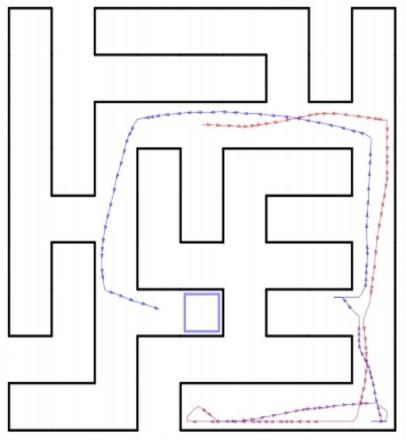
\includegraphics[height=0.42\textheight]{images/meta-rl-open/figures/maze-collect.jpg}\\[0.4em]
Collect $\mathcal{D}_{\text{tr}} \sim \pi^{\text{exp}}$
\end{column}
\begin{column}{0.45\textwidth}
\centering
{\footnotesize Learn policy that solves that MDP}\\[0.4em]
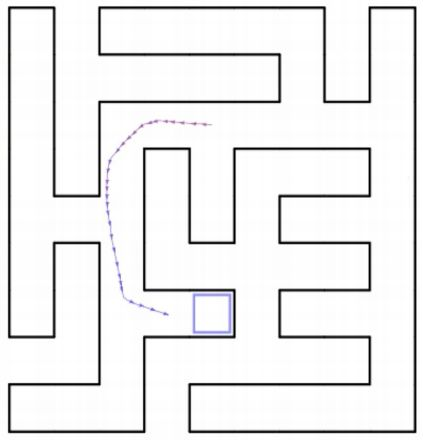
\includegraphics[height=0.42\textheight]{images/meta-rl-open/figures/maze-learn.jpg}\\[0.4em]
$\mathcal{D}_{\text{tr}} \rightarrow \pi^{\text{task}}$
\end{column}
\end{columns}
\vfill
{\scriptsize diagram adapted from Duan et al.\ '17}
\end{frame}

% ---------------------------------------------------------------- Slide 16
\begin{frame}{Meta-RL Example: Maze Navigation}
\begin{columns}[t]
\begin{column}{0.4\textwidth}
\textbf{Meta-Train Time:}\\
{\footnotesize Learn how to efficiently explore \& solve many MDPs:}\\[0.4em]
\centering
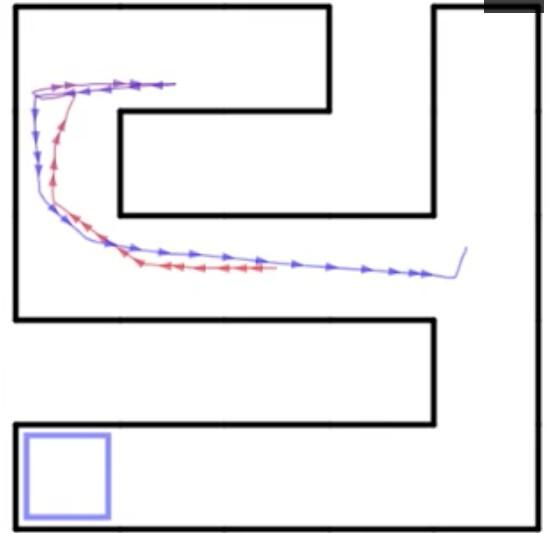
\includegraphics[height=0.26\textheight]{images/meta-rl-open/figures/maze-metatrain.jpg}\hfill
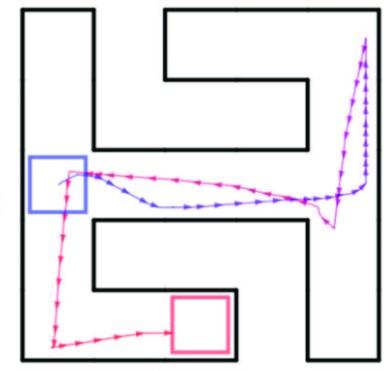
\includegraphics[height=0.22\textheight]{images/meta-rl-open/figures/maze-metatrain2.jpg}\hfill
\raisebox{2.2em}{$\cdots$ {\footnotesize\,meta-training tasks}}\\[0.4em]
{\footnotesize Meta-train $\pi^{\text{exp}},\, \pi^{\text{task}}$}
\end{column}
\begin{column}{0.58\textwidth}
\textbf{Meta-Test Time:}
\vspace{0.3em}

\begin{columns}[t]
\begin{column}{0.5\textwidth}
\centering
{\scriptsize Collect small amount of experience in new MDP}\\[0.3em]
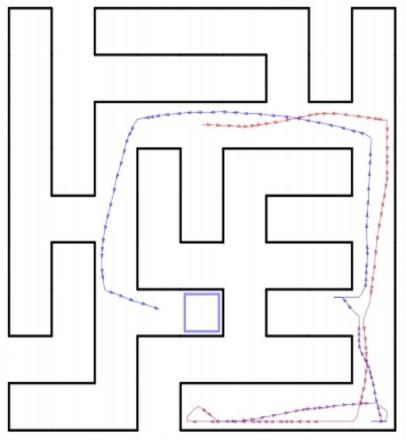
\includegraphics[height=0.26\textheight]{images/meta-rl-open/figures/maze-collect16.jpg}\\[0.3em]
{\footnotesize Collect $\mathcal{D}_{\text{tr}} \sim \pi^{\text{exp}}$}
\end{column}
\begin{column}{0.5\textwidth}
\centering
{\scriptsize Learn policy that solves that MDP}\\[0.3em]
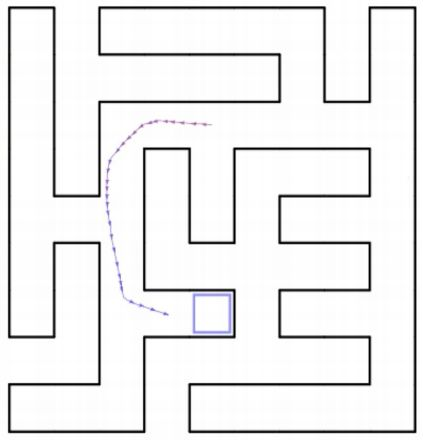
\includegraphics[height=0.26\textheight]{images/meta-rl-open/figures/maze-learn16.jpg}\\[0.3em]
{\footnotesize $\mathcal{D}_{\text{tr}} \rightarrow \pi^{\text{task}}$}
\end{column}
\end{columns}
\end{column}
\end{columns}
\vfill
\begin{center}\footnotesize
\textbf{Key assumption:} Meta-training \& meta-testing MDPs come from the same
distribution (so that we can expect generalization).
\end{center}
{\scriptsize diagram adapted from Duan et al.\ '17}
\end{frame}

% ---------------------------------------------------------------- Slide 17
\begin{frame}{The meta reinforcement learning problem}
\begin{columns}[t]
\begin{column}{0.5\textwidth}
\centering ``Generic'' learning:
\begin{align*}
    \theta^\star &= \arg\min_\theta \mathcal{L}(\theta, \mathcal{D}^{\text{tr}})\\
    &= f_{\text{learn}}(\mathcal{D}^{\text{tr}})
\end{align*}
\vspace{0.5em}

\centering Reinforcement learning:
\begin{align*}
    \theta^\star &= \arg\max_\theta \mathbb{E}_{\pi_\theta}\!\left[R(\tau)\right]\\
    &= f_{\text{RL}}(\mathcal{M}) \qquad \mathcal{M}=\{\mathcal{S},\mathcal{A},\mathcal{P},r\}
\end{align*}
\hspace{2.0em}\begin{tikzpicture}[baseline, inner sep=1pt,
    ar/.style={-{Stealth[length=1.6mm]}}]
    \node[font=\footnotesize\itshape] (lab) at (0,0) {MDP};
    \draw[ar] (lab.north) to[bend right=18] (0.5,0.75);
\end{tikzpicture}
\end{column}
\begin{column}{0.5\textwidth}
\centering ``Generic'' meta-learning:
\begin{align*}
    \theta^\star &= \arg\min_\theta \sum_{i=1}^{n} \mathcal{L}\!\left(\phi_i, \mathcal{D}^{\text{ts}}_i\right)\\
    \text{where } \phi_i &= f_\theta(\mathcal{D}^{\text{tr}}_i)
\end{align*}
\vspace{0.5em}

\centering Meta-reinforcement learning:
\begin{align*}
    \theta^\star &= \arg\max_\theta \sum_i \mathbb{E}_{\pi_{\phi_i}}\!\left[R(\tau)\right]\\
    \text{where } \phi_i &= f_\theta(\mathcal{M}_i)
\end{align*}
\hspace{3.0em}\begin{tikzpicture}[baseline, inner sep=1pt,
    ar/.style={-{Stealth[length=1.6mm]}}]
    \node[font=\footnotesize\itshape] (lab) at (0,0) {MDP for task $i$};
    \draw[ar] (lab.north) to[bend right=18] (-0.2,0.75);
\end{tikzpicture}
\end{column}
\end{columns}
\end{frame}

% ---------------------------------------------------------------- Slide 18
\begin{frame}{The meta reinforcement learning problem}
\begin{columns}[c]
\begin{column}{0.5\textwidth}
\[\resizebox{\linewidth}{!}{$\displaystyle
    \theta^\star = \arg\max_\theta \sum_i \mathbb{E}_{\pi_{\phi_i}}\!\left[R(\tau)\right],
        \;\; \phi_i = f_\theta(\mathcal{M}_i)$}\]
\footnotesize
assumption:\quad $\mathcal{M}_i \sim p(\mathcal{M})$
\vspace{0.6em}

meta test-time:\quad sample $\mathcal{M}_{\text{test}} \sim p(\mathcal{M})$,
get $\phi_i = f_\theta(\mathcal{M}_{\text{test}})$
\vspace{0.8em}

\begin{tikzpicture}[inner sep=1pt, ar/.style={-{Stealth[length=1.8mm]}}]
    \node (set) {$\{\mathcal{M}_1, \dots, \mathcal{M}_n\}$};
    \node[below left=0.55cm and -0.4cm of set, font=\scriptsize\itshape] (lbl) {meta-training MDPs};
    \draw[ar] (lbl) -- (set.south west);
\end{tikzpicture}
\end{column}
\begin{column}{0.5\textwidth}
\centering
\footnotesize Some examples:\\[0.3em]
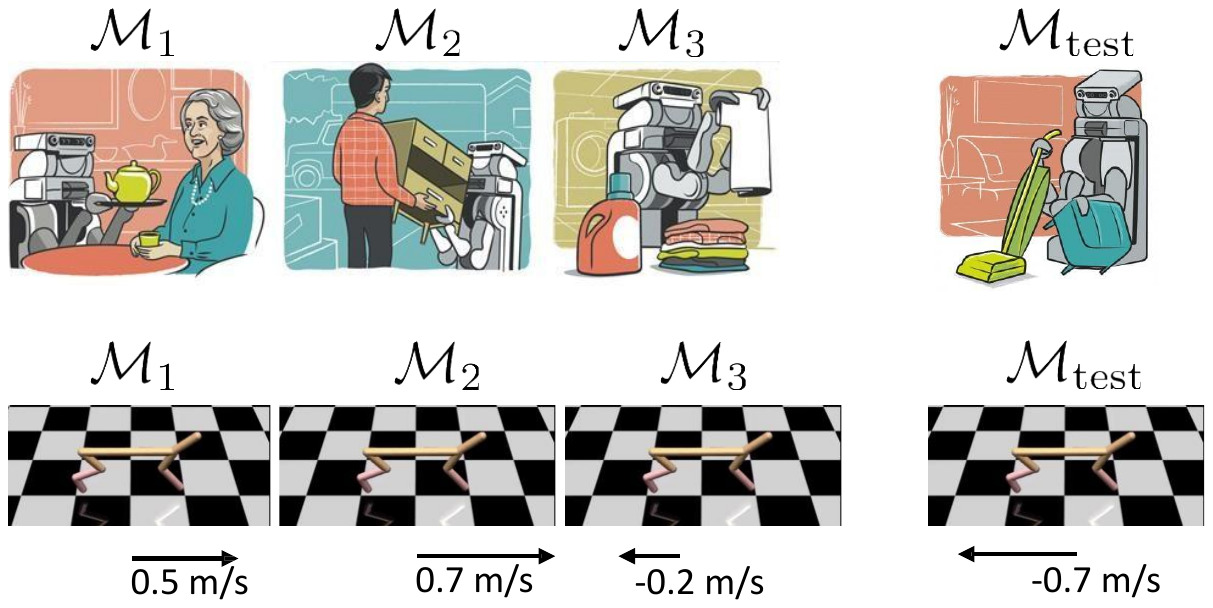
\includegraphics[width=\linewidth]{images/meta-rl-open/figures/examples-18.jpg}
\end{column}
\end{columns}
\end{frame}

% ---------------------------------------------------------------- Slide 19
\begin{frame}{Contextual policies and meta-learning}
\begin{columns}[c]
\begin{column}{0.38\textwidth}
\centering
$\displaystyle \theta^\star = \arg\max_\theta \sum_{i=1}^{n} \mathbb{E}_{\pi_{\phi_i}(\tau)}\!\left[R(\tau)\right]$\\[0.5em]
where $\phi_i = f_\theta(\mathcal{M}_i)$
\end{column}
\begin{column}{0.06\textwidth}
{\Large\color{green!55!black}$\boldsymbol{\Rightarrow}$}
\end{column}
\begin{column}{0.56\textwidth}
\centering
$\displaystyle \theta^\star = \arg\max_\theta \sum_{i=1}^{n} \mathbb{E}_{\pi_\theta}\!\left[R(\tau)\right]$\\[0.4em]
$\pi_\theta\big(a_t \mid \underbrace{s_t, s_1,a_1,r_1,\dots,s_{t-1},a_{t-1},r_{t-1}}\big)$\\[0.2em]
{\scriptsize context used to infer whatever we need to solve $\mathcal{M}_i$,\\
i.e., $z_t$ or $\phi_i$ (which are really the same thing)}
\end{column}
\end{columns}
\vfill
\begin{columns}[c]
\begin{column}{0.6\textwidth}
\footnotesize
in meta-RL, the \emph{context} is inferred from experience from $\mathcal{M}_i$
\vspace{0.4em}

in multi-task RL, the context is typically given
\end{column}
\begin{column}{0.4\textwidth}
\centering
\begin{tikzpicture}[inner sep=1pt, ar/.style={-{Stealth[length=1.8mm]}}]
    \node (pi) {$\pi_\theta(a_t \mid s_t,$};
    \node[right=0pt of pi] (ph) {$\phi_i$};
    \node[right=0pt of ph] (rb) {$)$};
    \node[below right=0.6cm and -0.2cm of ph, font=\scriptsize] (c) {``context''};
    \draw[ar] (c) -- (ph);
\end{tikzpicture}
\end{column}
\end{columns}
\vfill
\begin{columns}[c]
\begin{column}{0.33\textwidth}\centering
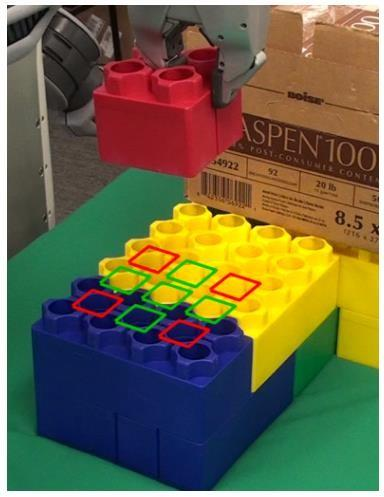
\includegraphics[height=0.22\textheight]{images/meta-rl-open/figures/ctx-stack.jpg}\\
{\footnotesize $\phi$: stack location}
\end{column}
\begin{column}{0.33\textwidth}\centering
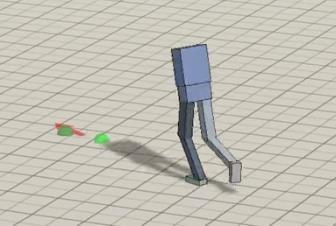
\includegraphics[height=0.22\textheight]{images/meta-rl-open/figures/ctx-walk.jpg}\\
{\footnotesize $\phi$: walking direction}
\end{column}
\begin{column}{0.33\textwidth}\centering
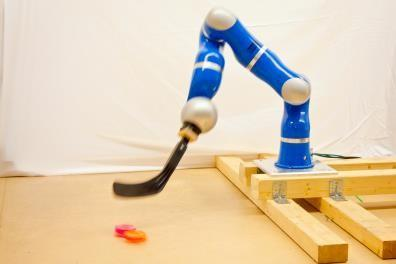
\includegraphics[height=0.22\textheight]{images/meta-rl-open/figures/ctx-puck.jpg}\\
{\footnotesize $\phi$: where to hit puck}
\end{column}
\end{columns}
\end{frame}

% ---------------------------------------------------------------- Slide 20
\begin{frame}{Meta-RL with recurrent policies}
\begin{columns}[T]
% ===================== left =====================
\begin{column}{0.42\textwidth}
\centering
$\displaystyle \theta^\star = \arg\max_\theta \sum_{i=1}^{n} \mathbb{E}_{\pi_{\phi_i}(\tau)}\!\left[R(\tau)\right]$\\[0.3em]
\tikz[baseline]{\node[draw=red, ellipse, inner sep=2pt]{where $\phi_i = f_\theta(\mathcal{M}_i)$};}
\vspace{0.8em}

\begin{tikzpicture}[ic/.style={inner sep=0},
    ba/.style={-{Stealth[length=3mm]}, line width=2.5pt, blue!45!black}]
    \node[ic] (ea) at (0,0)   {
\includegraphics[height=1.5cm]{images/meta-rl-open/figures/icons/earth.jpg}};
    \node[ic] (rb) at (2.6,0) {
\includegraphics[height=1.5cm]{images/meta-rl-open/figures/icons/robot.jpg}};
    \draw[ba] (ea.north) to[bend left=40] (rb.north);
    \draw[ba] (rb.south) to[bend left=40] (ea.south);
    \node[font=\footnotesize] at (1.3,1.5) {$r_t\quad s_{t+1}$};
    \node[font=\footnotesize] at (1.3,-1.5) {pick $a_t \sim \pi_\theta(a_t|s_t)$};
\end{tikzpicture}

\vspace{0.3em}
{\footnotesize use $(s_t,a_t,s_{t+1},r_t)$ to improve $\pi_\theta$}
\end{column}
% ===================== right =====================
\begin{column}{0.58\textwidth}
\footnotesize
main question: how to implement $f_\theta(\mathcal{M}_i)$? what should $f_\theta(\mathcal{M}_i)$ do?
\vspace{0.4em}

\tikz[baseline]{\node[draw=red, rounded corners, inner sep=3pt, align=left]{%
1.\ improve policy with experience from $\mathcal{M}_i$:\\
\hspace{1em}$\{(s_1,a_1,s_2,r_1),\dots,(s_T,a_T,s_{T+1},r_T)\}$};}
\vspace{0.3em}

2.\ (new in RL): choose how to interact, i.e.\ choose $a_t$ ---
meta-RL must also \emph{choose} how to \emph{explore!}
\vspace{0.5em}

\centering
\begin{tikzpicture}[bx/.style={draw, minimum width=0.6cm, minimum height=0.42cm},
    ar/.style={-{Stealth[length=1.3mm]}}, th/.style={-{Stealth[length=2mm]}, line width=1.1pt}]
    \node[bx] (b1) at (0,0) {}; \node[bx] (b2) at (1.75,0) {}; \node[bx] (b3) at (3.5,0) {};
    \node[bx] (b4) at (5.3,0) {};
    \node[font=\scriptsize] (t) at (0.1,1.1) {$\theta^\star$};
    \draw[th] (t) to[out=-80,in=90] (0.9,0.12);
    \draw[th] (t) to[out=0,in=90]   (2.6,0.12);
    \draw[th] (t) to[out=0,in=90]   (4.0,0.12);
    \draw[ar] (b1)--(b2); \draw[ar] (b2)--(b3);
    \draw[ar] (b3) -- node[above,font=\scriptsize]{$h_i$} (b4);
    \node[below=1pt of b1, font=\tiny] {$(s_1,a_1,s_2,r_1)$};
    \node[below=1pt of b2, font=\tiny] {$(s_2,a_2,s_3,r_2)$};
    \node[below=1pt of b3, font=\tiny] {$(s_3,a_3,s_4,r_3)$};
    \draw[ar] (b4.north)-- node[right,font=\scriptsize]{$a$} ++(0,0.55);
    \draw[ar] ([yshift=-0.55cm]b4.south)-- node[right,font=\scriptsize]{$s$} (b4.south);
    \node[below=0.6cm of b4, font=\scriptsize] {$\pi_{\phi_i}(a|s)$};
\end{tikzpicture}

\vspace{0.3em}
{\footnotesize as before, $\phi_i = [\,h_i,\ \theta_\pi\,]$}
\end{column}
\end{columns}
\end{frame}

% ---------------------------------------------------------------- Slide 21
\begin{frame}{Meta-RL with recurrent policies}
\begin{columns}[T]
\begin{column}{0.42\textwidth}
\centering
$\displaystyle \theta^\star = \arg\max_\theta \sum_{i=1}^{n} \mathbb{E}_{\pi_{\phi_i}(\tau)}\!\left[R(\tau)\right]$\\[0.4em]
where $\phi_i = f_\theta(\mathcal{M}_i)$
\vspace{0.8em}

\raggedright so\dots\ we just train an RNN policy?\\ yes!
\end{column}
\begin{column}{0.58\textwidth}
\centering
\begin{tikzpicture}[bx/.style={draw, minimum width=0.6cm, minimum height=0.42cm},
    ar/.style={-{Stealth[length=1.3mm]}}, th/.style={-{Stealth[length=2mm]}, line width=1.1pt}]
    \node[bx] (b1) at (0,0) {}; \node[bx] (b2) at (1.4,0) {}; \node[bx] (b3) at (2.8,0) {};
    \node[bx] (b4) at (4.4,0) {};
    \node[font=\scriptsize] (t) at (0.1,1.1) {$\theta^\star$};
    \draw[th] (t) to[out=-80,in=90] (0.7,0.12);
    \draw[th] (t) to[out=0,in=90]   (2.1,0.12);
    \draw[th] (t) to[out=0,in=90]   (3.5,0.12);
    \draw[ar] (b1)--(b2); \draw[ar] (b2)--(b3);
    \draw[ar] (b3) -- node[above,font=\scriptsize]{$h_i$} (b4);
    \node[below=1pt of b1, font=\tiny] {$(s_1,a_1,s_2,r_1)$};
    \node[below=1pt of b2, font=\tiny] {$(s_2,a_2,s_3,r_2)$};
    \node[below=1pt of b3, font=\tiny] {$(s_3,a_3,s_4,r_3)$};
    \draw[ar] (b4.north)-- node[right,font=\scriptsize]{$a$} ++(0,0.5);
    \draw[ar] ([yshift=-0.5cm]b4.south)-- node[right,font=\scriptsize]{$s$} (b4.south);
    \node[below=0.55cm of b4, font=\scriptsize] {$\pi_{\phi_i}(a|s)$};
\end{tikzpicture}
\end{column}
\end{columns}
\vfill
\begin{center}
\textbf{crucially}, RNN hidden state is \textbf{not} reset between episodes!
\end{center}
\vfill
\begin{center}
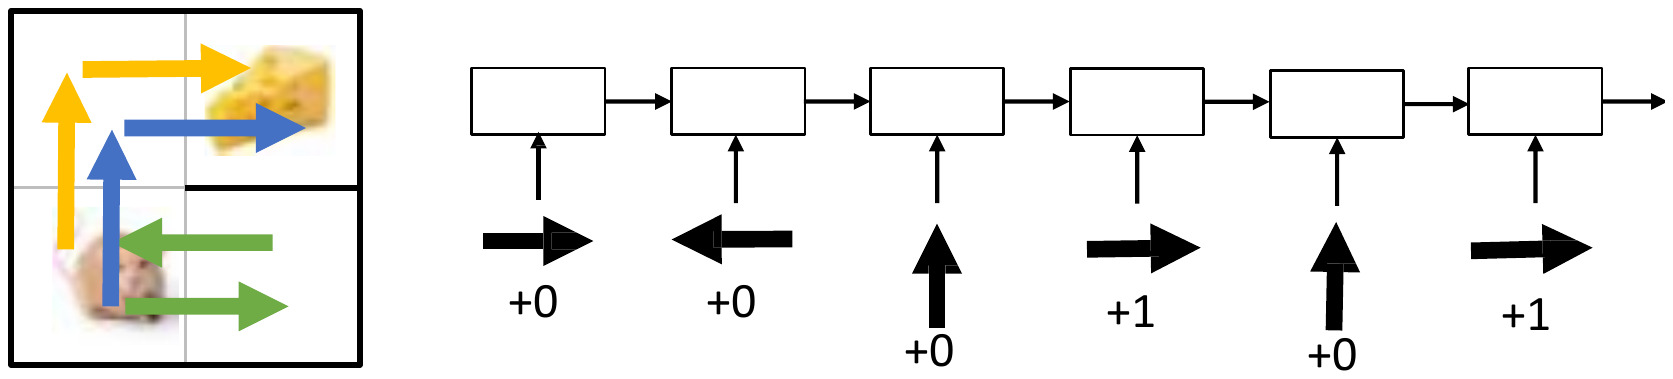
\includegraphics[width=0.95\linewidth]{images/meta-rl-open/figures/s21-unroll.jpg}
\end{center}
\end{frame}

% ---------------------------------------------------------------- Slide 22
\begin{frame}{Why recurrent policies learn to explore}
\begin{columns}[T]
\begin{column}{0.4\textwidth}
\centering
\resizebox{\linewidth}{!}{%
\begin{tikzpicture}[bx/.style={draw, minimum width=0.55cm, minimum height=0.4cm},
    ar/.style={-{Stealth[length=1.3mm]}}, th/.style={-{Stealth[length=2mm]}, line width=1.1pt}]
    \node[bx] (b1) at (0,0) {}; \node[bx] (b2) at (1.25,0) {}; \node[bx] (b3) at (2.5,0) {};
    \node[bx] (b4) at (3.9,0) {};
    \node[font=\scriptsize] (t) at (0.1,1.05) {$\theta^\star$};
    \draw[th] (t) to[out=-80,in=90] (0.62,0.12);
    \draw[th] (t) to[out=0,in=90]   (1.88,0.12);
    \draw[th] (t) to[out=0,in=90]   (3.1,0.12);
    \draw[ar] (b1)--(b2); \draw[ar] (b2)--(b3);
    \draw[ar] (b3) -- node[above,font=\scriptsize]{$h_i$} (b4);
    \node[below=1pt of b1, font=\tiny] {$(s_1,a_1,s_2,r_1)$};
    \node[below=1pt of b2, font=\tiny] {$(s_2,a_2,s_3,r_2)$};
    \node[below=1pt of b3, font=\tiny] {$(s_3,a_3,s_4,r_3)$};
    \draw[ar] (b4.north)-- node[right,font=\scriptsize]{$a$} ++(0,0.5);
    \draw[ar] ([yshift=-0.5cm]b4.south)-- node[right,font=\scriptsize]{$s$} (b4.south);
    \node[below=0.55cm of b4, font=\scriptsize] {$\pi_{\phi_i}(a|s)$};
\end{tikzpicture}}
\end{column}
\begin{column}{0.6\textwidth}
\footnotesize
\begin{enumerate}
    \item improve policy with experience from $\mathcal{M}_i$:\\
          \resizebox{0.95\linewidth}{!}{$\{(s_1,a_1,s_2,r_1),\dots,(s_T,a_T,s_{T+1},r_T)\}$}
    \item (new in RL): choose how to interact, i.e.\ choose $a_t$\\
          meta-RL must also \emph{choose} how to \emph{explore!}
\end{enumerate}
\[ \theta^\star = \arg\max_\theta \mathbb{E}_{\pi_\theta}\!\left[\sum_{t=0}^{T} r(s_t,a_t)\right] \]
\end{column}
\end{columns}
\vfill
\begin{columns}[c]
\begin{column}{0.14\textwidth}
\centering
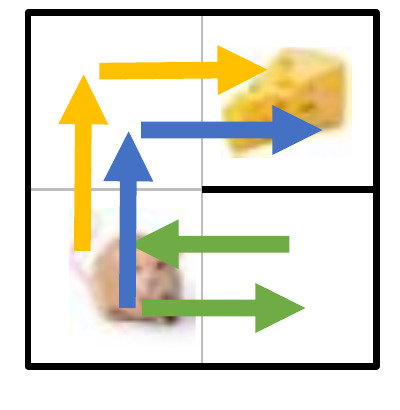
\includegraphics[width=\linewidth]{images/meta-rl-open/figures/s22-maze.jpg}
\end{column}
\begin{column}{0.46\textwidth}
\centering
\resizebox{\linewidth}{!}{%
\begin{tikzpicture}[font=\scriptsize,
    g/.style={-{Stealth[length=2.4mm]}, line width=2.5pt, green!60!black},
    b/.style={-{Stealth[length=2.4mm]}, line width=2.5pt, blue!70},
    yl/.style={-{Stealth[length=2.4mm]}, line width=2.5pt, yellow!85!black},
    br/.style={decorate, decoration={brace, amplitude=4pt, mirror}}]
    % episode / meta-episode arrows
    \draw[g] (0.0,0.5)--(0.9,0.5);
    \draw[g] (1.9,0.5)--(1.0,0.5);
    \draw[b] (2.3,0.1)--(2.3,0.9);
    \draw[b] (2.7,0.5)--(3.6,0.5);
    \draw[yl] (4.0,0.1)--(4.0,0.9);
    \draw[yl] (4.4,0.5)--(5.3,0.5);
    \draw[br] (-0.05,-0.1)--(1.95,-0.1) node[midway,below=4pt]{episode};
    \draw[br] (-0.05,-0.9)--(5.35,-0.9) node[midway,below=4pt]{meta-episode};
\end{tikzpicture}}
\end{column}
\begin{column}{0.37\textwidth}
\footnotesize
optimizing total reward over the entire \textbf{meta-episode} with RNN policy
\textbf{automatically} learns to explore!
\end{column}
\end{columns}
\end{frame}

% ---------------------------------------------------------------- Slide 23
\begin{frame}{Black-Box Meta-RL: Algorithm}
\textbf{Meta-Training}
\begin{enumerate}
    \item Sample task $\mathcal{T}_i$
    \item Roll-out policy $\pi(a \mid s, \mathcal{D}^{\text{tr}}_i)$ for $N$ episodes
          \hfill {\footnotesize(under dynamics $p_i(s'\!\mid s,a)$ and reward $r_i(s,a)$)}
    \item Store sequence in replay buffer for task $\mathcal{T}_i$
    \item Update policy to maximize discounted return for all tasks.
    \item \textbf{Repeat} (go back to step 1).
\end{enumerate}
\vspace{0.5em}
\textbf{Meta-Test Time}
\begin{enumerate}
    \item Sample new task $\mathcal{T}_j$
    \item Roll-out policy $\pi(a \mid s, \mathcal{D}^{\text{tr}}_j)$ for up to $N$ episodes
\end{enumerate}
\end{frame}

% ---------------------------------------------------------------- Slide 24
\begin{frame}{Meta-RL Example}
\centering
{\footnotesize Experiment: Learning to visually navigate a maze --- train on 1000 small
mazes, test on held-out small mazes and large mazes}
\vfill
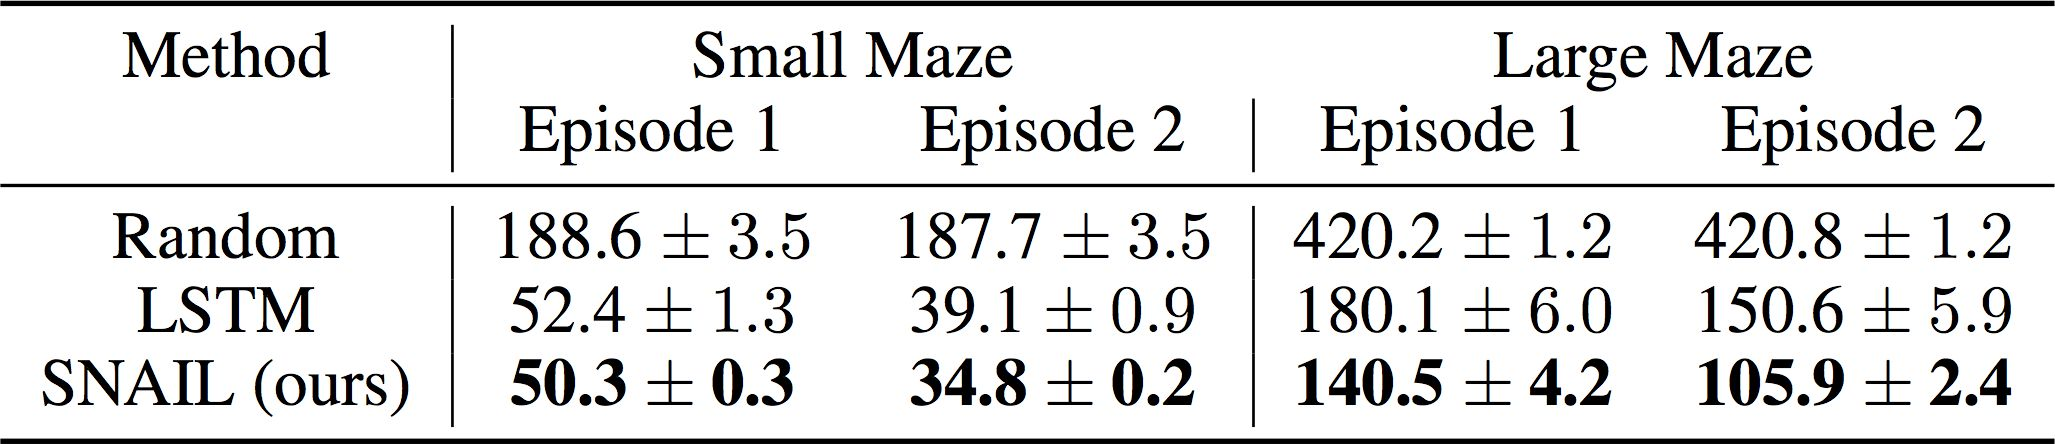
\includegraphics[width=\linewidth,keepaspectratio]{images/meta-rl-open/figures/snail-maze.jpg}
\vfill
{\scriptsize From: Mishra, Rohaninejad, Chen, Abbeel. A Simple Neural Attentive
Meta-Learner. ICLR 2018}
\end{frame}

% ---------------------------------------------------------------- Slide 25
\begin{frame}{Meta-RL with recurrent policies}
\centering
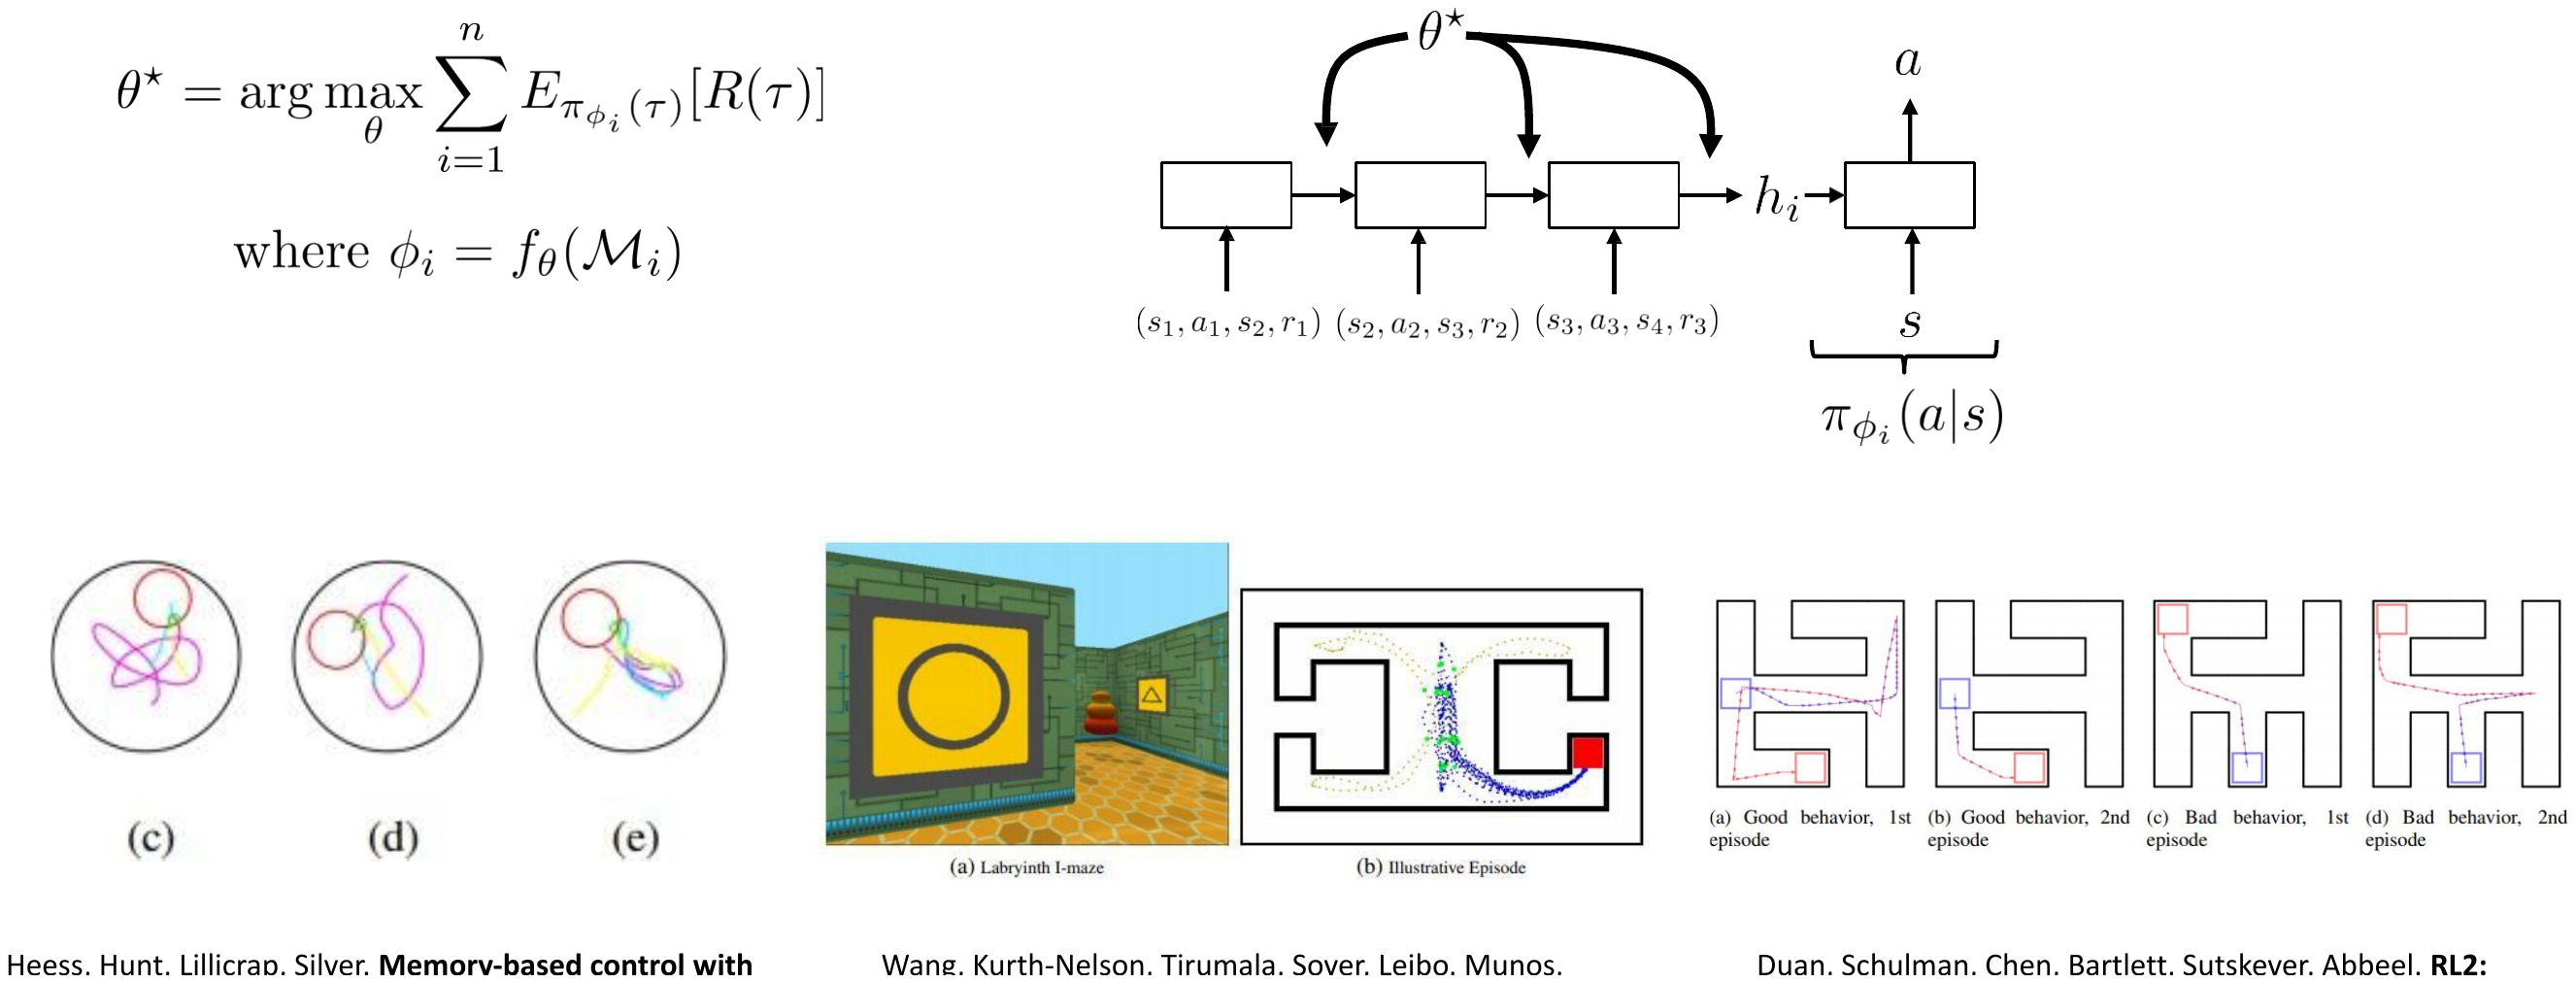
\includegraphics[width=\linewidth,height=0.66\textheight,keepaspectratio]{images/meta-rl-open/figures/arch-papers.jpg}
\vfill
{\tiny Heess et al. Memory-based control with recurrent neural networks. 2015. \;\textbullet\;
Wang et al. Learning to Reinforcement Learn. 2016. \;\textbullet\;
Duan, Schulman, Chen, Bartlett, Sutskever, Abbeel. RL$^2$: Fast Reinforcement Learning
via Slow Reinforcement Learning. 2016.}
\end{frame}

% ---------------------------------------------------------------- Slide 26
\begin{frame}{Architectures for meta-RL}
\centering
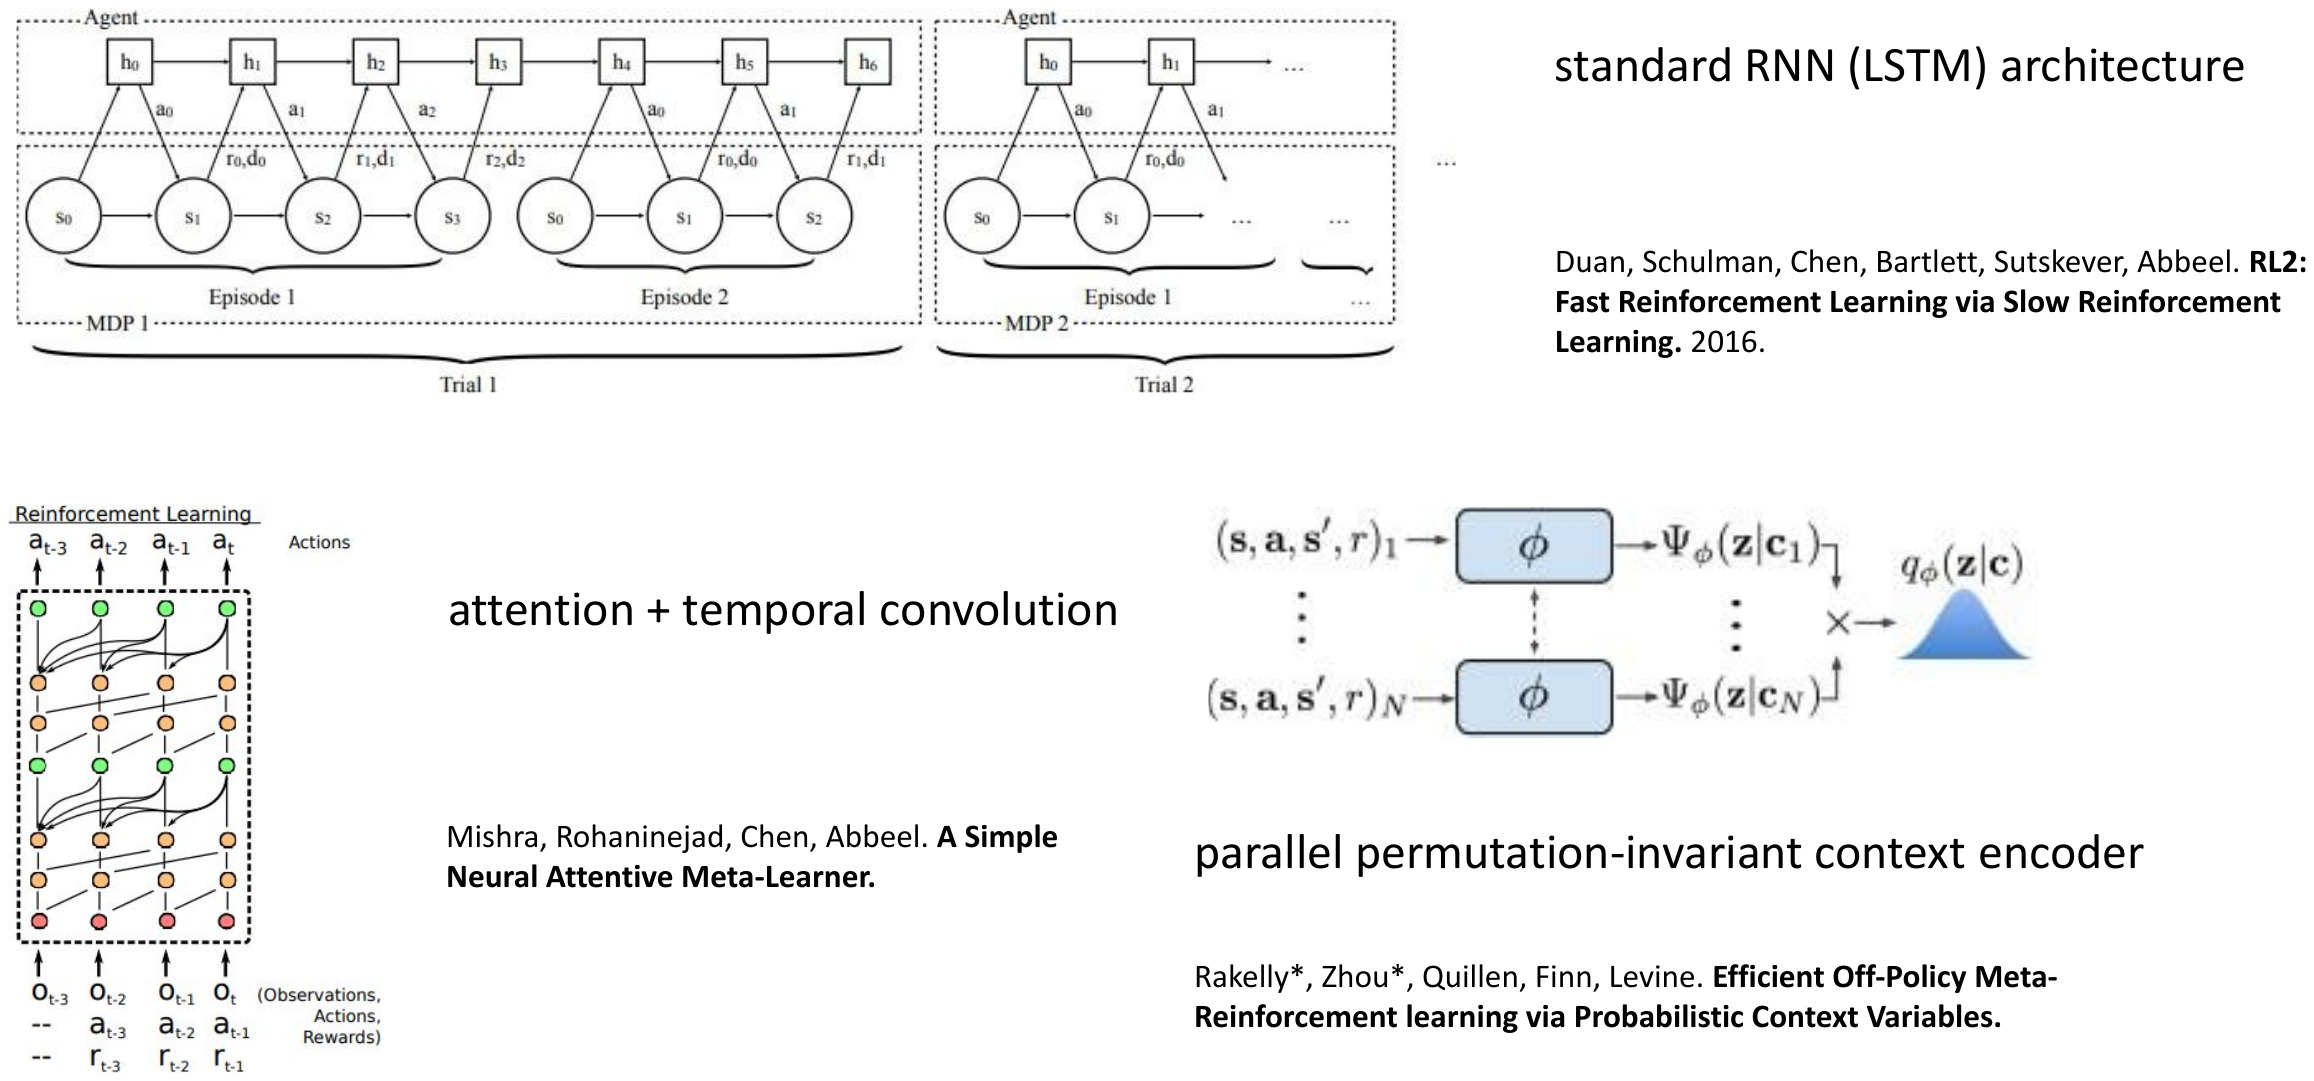
\includegraphics[width=\linewidth,height=0.74\textheight,keepaspectratio]{images/meta-rl-open/figures/arch-meta-rl.jpg}
\end{frame}
